\begin{frame}
	\centering \LARGE \color{naranjaUCA} Modelo de cola M/M/s
			\begin{center}
				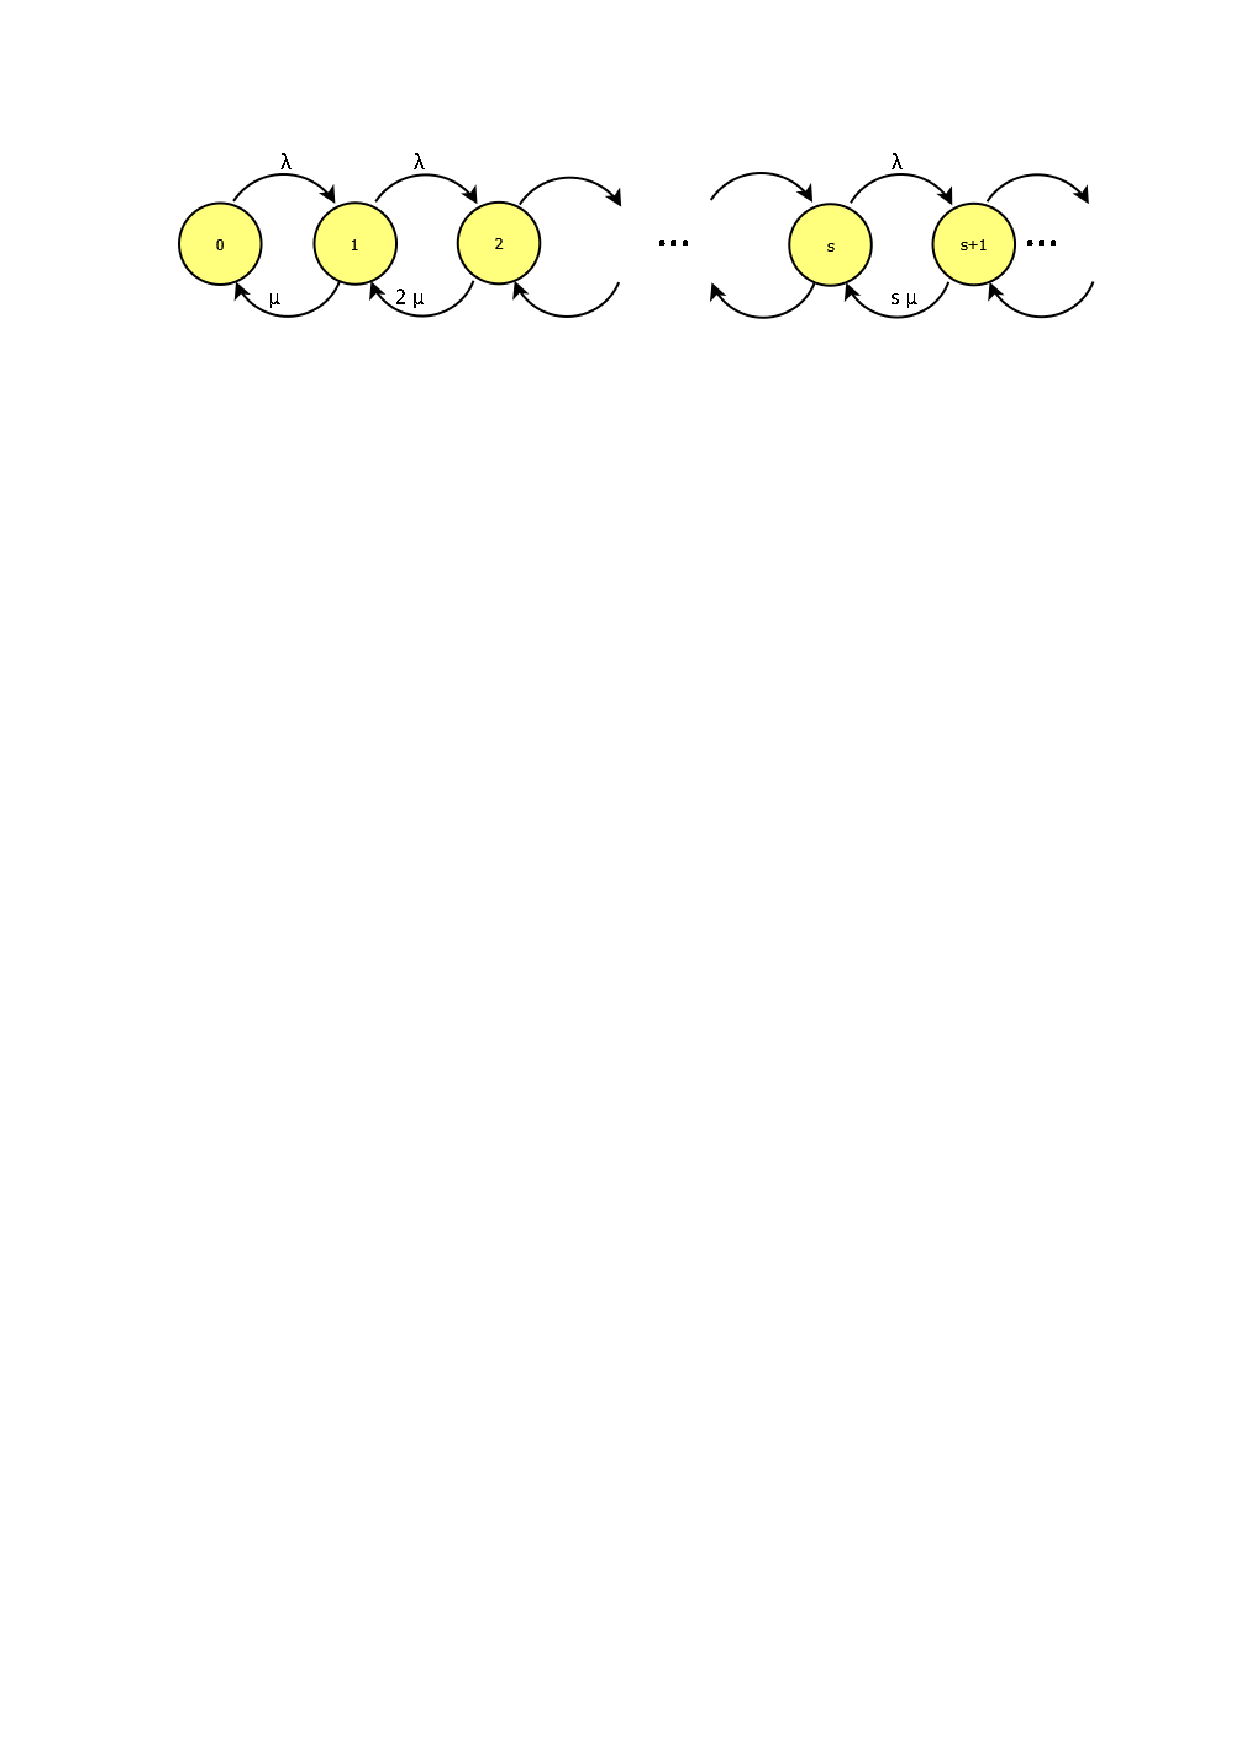
\includegraphics[trim = 10mm 220mm 10mm 25mm, clip,width=0.9\linewidth]{MMs}
			\end{center}
\end{frame}
\begin{frame}{M/M/s}
	Cuando en el sistema haya $j\leq s$ clientes, todos estar\'an siendo servidos. Cuando haya $j>s$, los que vayan llegando esperar\'an en la cola. \\
	\pause
	
	Este tipo de cola se puede modelizar como un proceso de nacimiento-muerte con los siguientes par\'ametros
	
	\pause
		$$\begin{array}{cc}
		\lambda_j=\lambda & (j=0,1,2,...)\\
		\mu_j=j\mu & (j=1,2,...,s)\\
		\mu_j=s\mu & (j=s+1,s+2,...)\\
		\end{array}$$
	\pause
	Definimos $\rho=\displaystyle\frac{\lambda}{s\mu}$.
	\\ 
	\pause
	Asumiendo $\rho\geq1$ 
\end{frame}

\begin{frame}{M/M/s}
	Usando las ecuaciones de equilibrio:
	$$\begin{array}{cc}
	\pi_0=\displaystyle\frac{1}{\displaystyle \sum_{t=0}^{t=s-1}\frac{(s\rho)^t}{t!}+\frac{(s\rho)s}{s!(1-\rho)}} & \\
	\pi_j=\displaystyle\frac{(s\rho)^j\pi_0}{j!} & (j=0,1,...,s)\\
	\pi_j=\displaystyle\frac{(s\rho)^j\pi_0}{s!s^{j-s}} & (j=s+1,s+2,...)\\
	\end{array}$$
	
	\pause
	La probabilidad de que todos los servidores est\'en ocupados, que viene dada por:
	$$P(j\geq s)=\sum_{k\geq s}^{}\pi_k=\frac{(s\rho)^s}{s!(1-\rho)}\pi_0$$
	$$L_q=\frac{P(j\geq s)\rho}{1-\rho}$$
\end{frame}

\begin{frame}{M/M/s}
	Por las fórmulas de Little obtenemos:		$$W_q=\frac{L_q}{\lambda}=\frac{P(j\geq s)}{s\mu-\lambda}$$
	\pause
	Una vez que el cliente est\'a en el servidor, como este sigue una distribuci\'on exponencial, tenemos que $W_s=\frac{1}{\mu}$ \pause
	$$L=L_q+L_s=L_q+\frac{\lambda}{\mu}$$
	\pause
	Por Little:
	$$W=\frac{L}{\lambda}=\frac{L_q}{\lambda}+\frac{1}{\mu}$$
\end{frame}